\documentclass[tikz]{standalone}
\usepackage{pgfplots}
\pgfplotsset{compat=1.15}
\usepackage{mathrsfs}
\usetikzlibrary{arrows,calc}
\usepackage{tkz-euclide}
\pagestyle{empty}

\definecolor{AngleClr}{rgb}{0,0.39215686274509803,0}
\definecolor{ShapeClr}{rgb}{0.6,0.2,0}
\definecolor{BlueSqr}{RGB}{5,81,163}
\definecolor{RedSqr}{RGB}{0, 156, 0}

\begin{document}

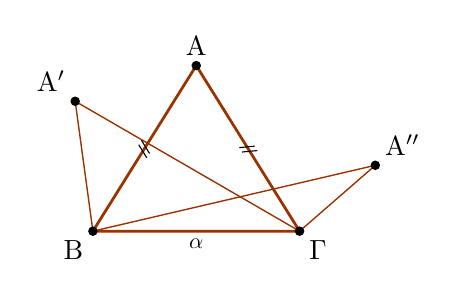
\begin{tikzpicture}[scale=.75]
\tkzSetUpLine[line width=1pt,color=black]
\tkzSetUpPoint[fill=black]

\tkzDefPoints{0/0/B,3.5/0/C,-0.3/2.2/A}

\tkzCalcLength(A,B)\tkzGetLength{dAB}
\tkzCalcLength(A,C)\tkzGetLength{dAC}

\pgfmathsetmacro{\dOne}{(\dAB + \dAC)/2}

\tkzInterCC[R](B,\dOne)(C,\dOne) \tkzGetPoints{D}{X}

\pgfmathsetmacro{\dTwo}{\dAB + \dAC - 1.7}
\tkzInterCC[R](B,\dTwo)(C,1.7) \tkzGetPoints{E}{X}

% \tkzInterCC[R](A,\dOne)(C,\dOne) \tkzGetPoints{X}{B'}
% \tkzInterCC[R](A,\dOne)(C,\dOne) \tkzGetPoints{X}{B'}


\tkzFillPolygon[fill=white](A,B,C)
\tkzFillPolygon[fill=white](D,B,C)
\tkzFillPolygon[fill=white](E,B,C)

\tkzDrawPolygon[line width=0.5pt,color=ShapeClr](A,B,C)
\tkzDrawPolygon[color=ShapeClr](D,B,C)
\tkzDrawPolygon[line width=0.5pt,color=ShapeClr](E,B,C)

\tkzDrawPoints[size=3](A,B,C,D,E)
\tkzLabelPoint[above left](A){$\rm A'$}
\tkzLabelPoint[above](D){$\rm A$}
\tkzLabelPoint[above right](E){$\rm A''$}
\tkzLabelPoint[below left](B){$\rm B$}
\tkzLabelPoint[below right](C){$\rm \Gamma$}

\tkzMarkSegments[mark=s||,size=2.5](D,B D,C)
\tkzLabelSegment[scale=0.8](B,C){$\alpha$}
\end{tikzpicture}

\end{document}
